\documentclass[a4paper,11pt]{article}
\usepackage{zh_CN-Adobefonts_external} % Simplified Chinese Support using
\usepackage{fancyhdr}  % 页眉页脚
\usepackage{minted}    % 代码高亮
\usepackage{graphicx}  %图片
\usepackage{pdfpages}  %pdf
\usepackage[colorlinks]{hyperref}  % 目录可跳转
\setlength{\headheight}{15pt}


% 定义页眉页脚
\pagestyle{fancy}
\fancyhf{}
\fancyhead[C]{Algorithm Template by lxz}
\lfoot{}
\cfoot{\thepage}
\rfoot{}

\author{lxz}   
\title{Algorithm template}

\begin{document} 
\maketitle % 封面
\newpage % 换页
\tableofcontents % 目录
\newpage
\section{基础算法} % 一级标题
\subsection{高精度} % 二级标题
\subsubsection{高精/低精} % 三级标题
\inputminted[breaklines]{c++}{基础算法/高精除低精.cpp} % 插入代码文件
\subsection{差分} % 二级标题
\subsubsection{差分矩阵} % 三级标题
\inputminted[breaklines]{c++}{基础算法/差分矩阵.cpp}

\newpage
\section{经典动态规划}
\subsection{数位dp} % 二级标题
\inputminted[breaklines]{c++}{经典动态规划/数位dp.cpp}
\subsection{最长上升子序列LIS} % 二级标题
\inputminted[breaklines]{c++}{经典动态规划/LIS.cpp}
\subsection{背包} % 二级标题
\subsubsection{01背包} % 三级标题
\inputminted[breaklines]{c++}{经典动态规划/01背包.cpp}
\subsubsection{完全背包} % 三级标题
\inputminted[breaklines]{c++}{经典动态规划/完全背包.cpp}
\subsubsection{多重背包(普通和二进制拆位)} % 三级标题
\inputminted[breaklines]{c++}{经典动态规划/多重背包.cpp}
\subsubsection{分组背包} % 三级标题
\inputminted[breaklines]{c++}{经典动态规划/分组背包.cpp}
\subsection{最长公共子序列} % 二级标题
\inputminted[breaklines]{c++}{经典动态规划/最长公共子序列.cpp}
\subsection{单调队列优化dp} % 二级标题
\inputminted[breaklines]{c++}{经典动态规划/单调队列优化dp.cpp}

\newpage
\section{搜索} % 一级标题
\subsection{模拟退火} % 二级标题
\inputminted[breaklines]{c++}{搜索/模拟退火.cpp}

\newpage
\section{图论} % 一级标题
\subsection{树的重心(一棵树的和每个子树的)}
\inputminted[breaklines]{c++}{图论/树的重心.cpp}
\subsection{差分约束}
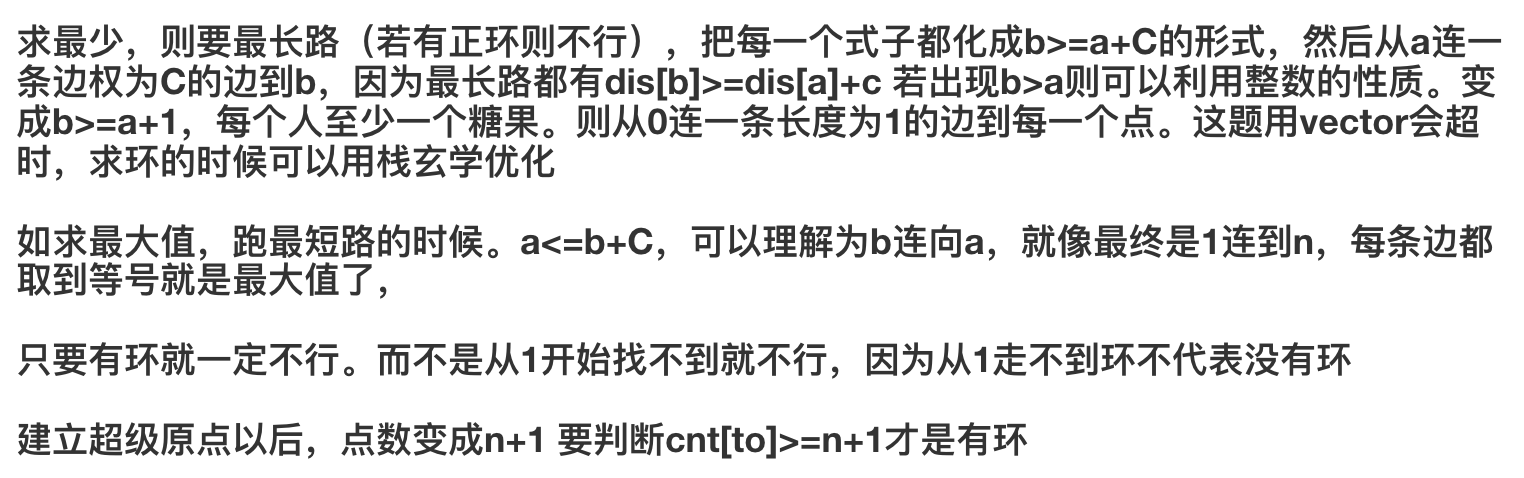
\includegraphics[scale=0.6]{图论/差分1.png}
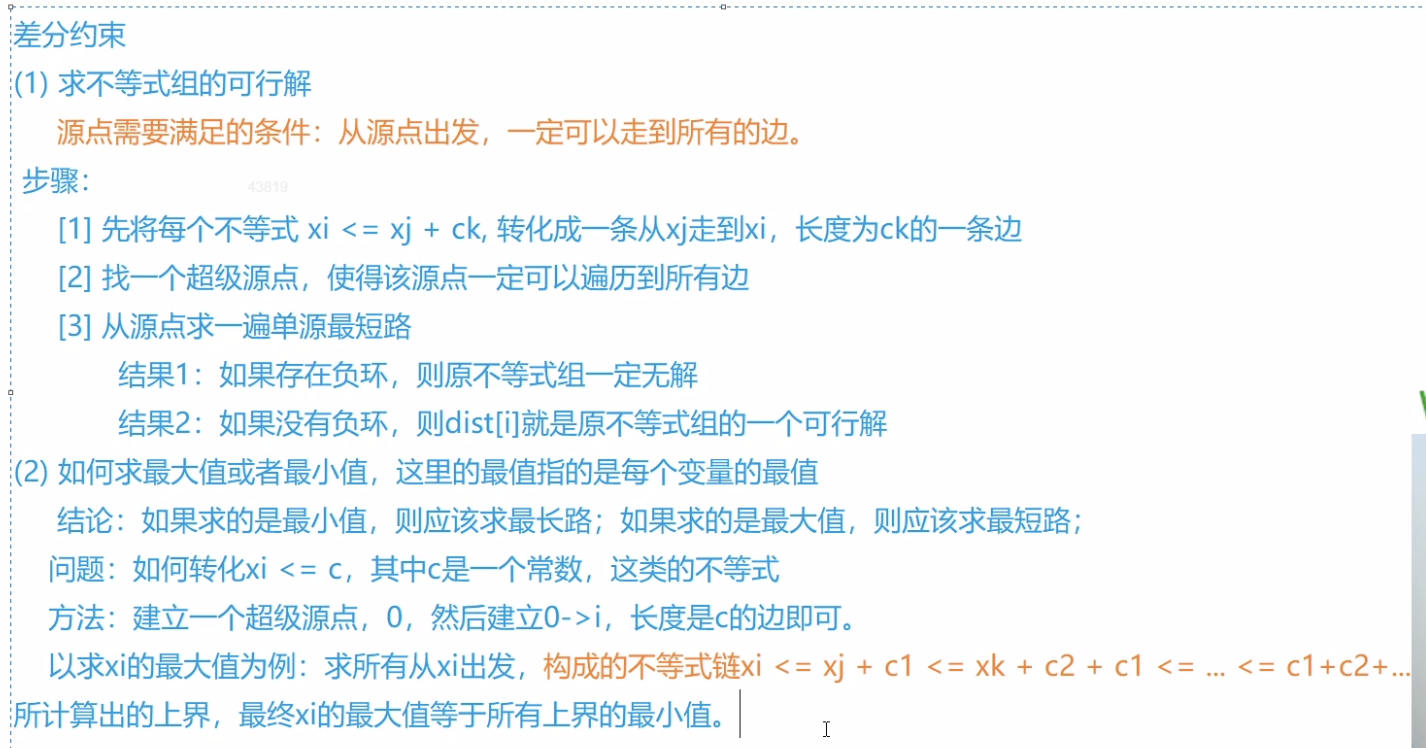
\includegraphics[scale=0.6]{图论/差分2.png}
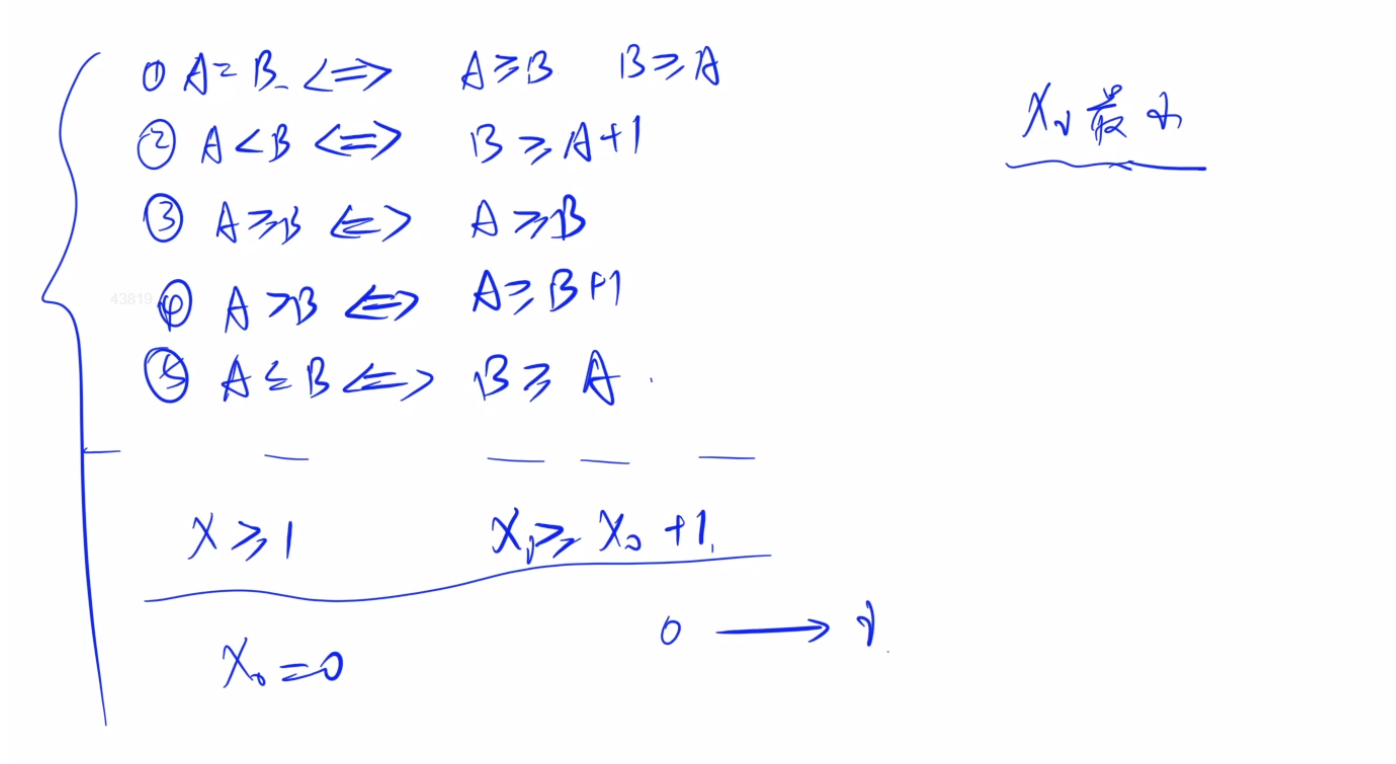
\includegraphics[scale=0.6]{图论/差分3.png}
\inputminted[breaklines]{c++}{图论/差分约束.cpp}
\subsection{欧拉路径和欧拉回路}
\subsubsection{欧拉回路和路径判定} % 三级标题
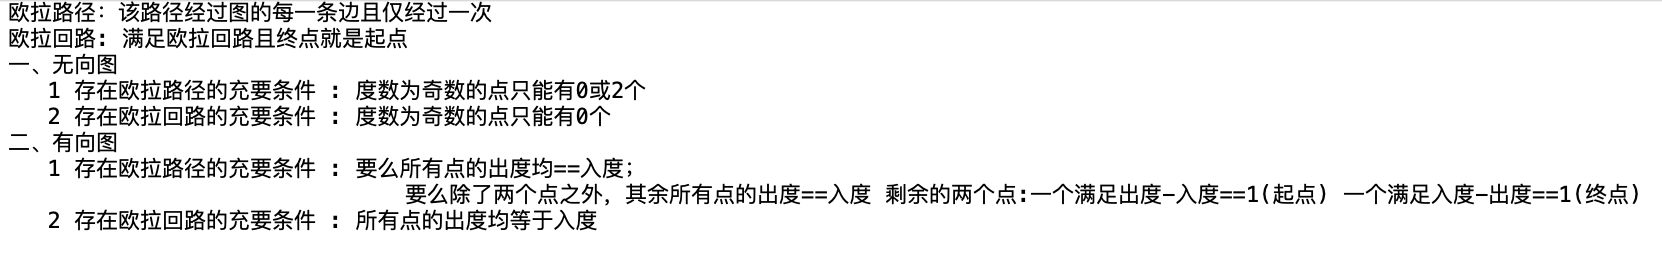
\includegraphics[scale=0.6]{图论/欧拉.png}
\subsubsection{欧拉回路输出路径} % 三级标题
\inputminted[breaklines]{c++}{图论/欧拉回路输出路径.cpp}
\subsection{网络流} % 二级标题
\subsubsection{最大流} % 三级标题
\inputminted[breaklines]{c++}{图论/最大流.cpp} % 插入代码文件
\subsubsection{无源汇上下界可行流} % 三级标题
\inputminted[breaklines]{c++}{图论/无源汇上下界最大流.cpp} % 插入代码文件
\subsubsection{费用流} % 三级标题
\inputminted[breaklines]{c++}{图论/费用流.cpp} % 插入代码文件
\subsection{最小生成树} % 二级标题
\subsubsection{Kruskal} % 三级标题
\inputminted[breaklines]{c++}{图论/Kruskal.cpp} % 插入代码文件
\subsection{2Sat} % 二级标题
\inputminted[breaklines]{c++}{图论/2sat.cpp} % 插入代码文件
\subsection{lca} % 二级标题
\inputminted[breaklines]{c++}{图论/lca.cpp} % 插入代码文件
\subsection{拓扑排序}
\inputminted[breaklines]{c++}{图论/拓扑排序.cpp}
\subsection{多源最短路}
\subsubsection{Floyd}
\inputminted[breaklines]{c++}{图论/多源最短路.cpp}
\subsubsection{Floyd求最小环}
\inputminted[breaklines]{c++}{图论/floyd求最小环.cpp}
\subsection{单源最短路}
\subsubsection{SPFA}
\inputminted[breaklines]{c++}{图论/spfa.cc}
\subsubsection{堆优化dij}
\inputminted[breaklines]{c++}{图论/堆优化dij.cpp}
\subsubsection{SPFA判负环}
\inputminted[breaklines]{c++}{图论/spfa判负环.cpp}

\subsection{有向图强连通分量}
\subsubsection{scc tarjan}
\inputminted[breaklines]{c++}{图论/scc_tarjan.cpp}
\subsection{无向图双连通分量}
\subsubsection{边双联通分量}
\inputminted[breaklines]{c++}{图论/边双联通分量.cpp}
\subsubsection{点双联通分量}
\inputminted[breaklines]{c++}{图论/点双联通分量.cpp}
\subsection{二分图}
\subsubsection{染色法判定二分图}
\inputminted[breaklines]{c++}{图论/染色法.cpp}
\subsubsection{最大匹配=最小点覆盖:选出最少的点,使每条边至少有一个点被选出来(在选出的点里面)=点数-最大独立集:选出最多的点使得选出的点之间没有边。=点数-最小路径点覆盖(最小路径覆盖):针对一个有向无环图(DAG),用最少条互不相交路径,覆盖所有点。(其中互不相交是指点不重复)(匈牙利算法 $O(n*m)$ )}
\inputminted[breaklines]{c++}{图论/匈牙利算法.cpp}

\newpage
\section{数据结构} % 一级标题
\subsection{链表} % 二级标题
\inputminted[breaklines]{c++}{数据结构/链表.cpp}
\subsection{字典树} % 二级标题
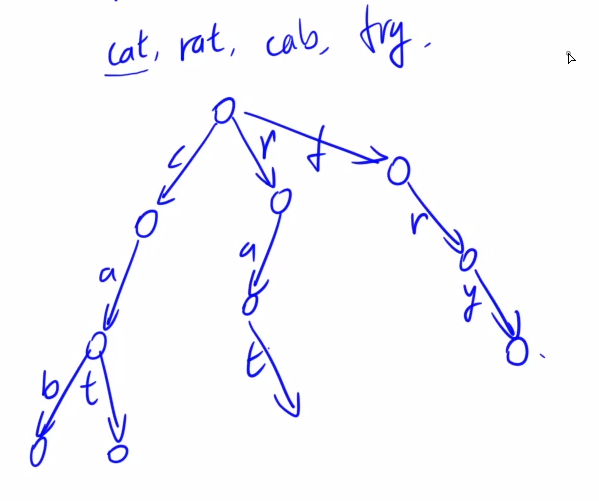
\includegraphics[scale=0.6]{数据结构/trie.png}
\inputminted[breaklines]{c++}{数据结构/字典树.cpp}
\subsection{可撤销并查集} % 二级标题
\inputminted[breaklines]{c++}{数据结构/可撤销并查集.cpp}
\subsection{线段树} % 二级标题
\subsubsection{单点修改} % 三级标题
\inputminted[breaklines]{c++}{数据结构/单点线段树.cpp}
\subsubsection{区间修改} % 三级标题
\inputminted[breaklines]{c++}{数据结构/区间线段树.cpp}
\subsubsection{返回node的线段树(区间最大字段和)} % 三级标题
\inputminted[breaklines]{c++}{数据结构/返回node的线段树.cpp}
\subsubsection{括号序列线段树(区间括号序列是否合法)} % 三级标题
\inputminted[breaklines]{c++}{数据结构/括号序列线段树.cpp}
\subsection{可持久化数据结构(历史版本)} % 二级标题
\subsubsection{主席树第K小数} % 三级标题
\inputminted[breaklines]{c++}{数据结构/主席树.cpp}
\subsubsection{可持久化trie求L-R中某个后缀与X最大异或和} % 三级标题
\inputminted[breaklines]{c++}{数据结构/可持久化trie.cpp}
\subsection{树套树} % 二级标题
\subsubsection{线段树套线段树求区间max,sum,min} % 三级标题
\inputminted[breaklines]{c++}{数据结构/线段树套线段树求区间max,sum,min.cpp}
\subsection{树状数组} % 二级标题
\inputminted[breaklines]{c++}{数据结构/树状数组.cpp}
\subsection{RMQ(st表)} % 二级标题
\inputminted[breaklines]{c++}{数据结构/RMQ.cpp}
\subsection{单调队列} % 二级标题
\inputminted[breaklines]{c++}{数据结构/单调队列.cpp}
\subsection{点分治} % 二级标题
\inputminted[breaklines]{c++}{数据结构/点分治.cpp}
\subsection{树链剖分} % 二级标题
\inputminted[breaklines]{c++}{数据结构/树链剖分.cpp}
\subsection{Splay} % 二级标题
\inputminted[breaklines]{c++}{数据结构/Splay.cpp}
\subsection{莫队} % 二级标题
\subsubsection{基础莫队} % 三级标题
\inputminted[breaklines]{c++}{数据结构/莫队.cpp}
\subsubsection{带修莫队} % 三级标题
\inputminted[breaklines]{c++}{数据结构/带修莫队.cpp}

\newpage
\section{数论} % 一级标题
\subsection{阶乘分解} % 二级标题
\inputminted[breaklines]{c++}{数论/阶乘分解.cpp}
\subsection{扩展中国剩余定理} % 二级标题
\inputminted[breaklines]{c++}{数论/扩展中国剩余定理.cpp}
\subsection{min25求1e10以内素数和} % 二级标题
\inputminted[breaklines]{c++}{数论/min25.cpp}
\subsection{矩阵快速幂} % 二级标题
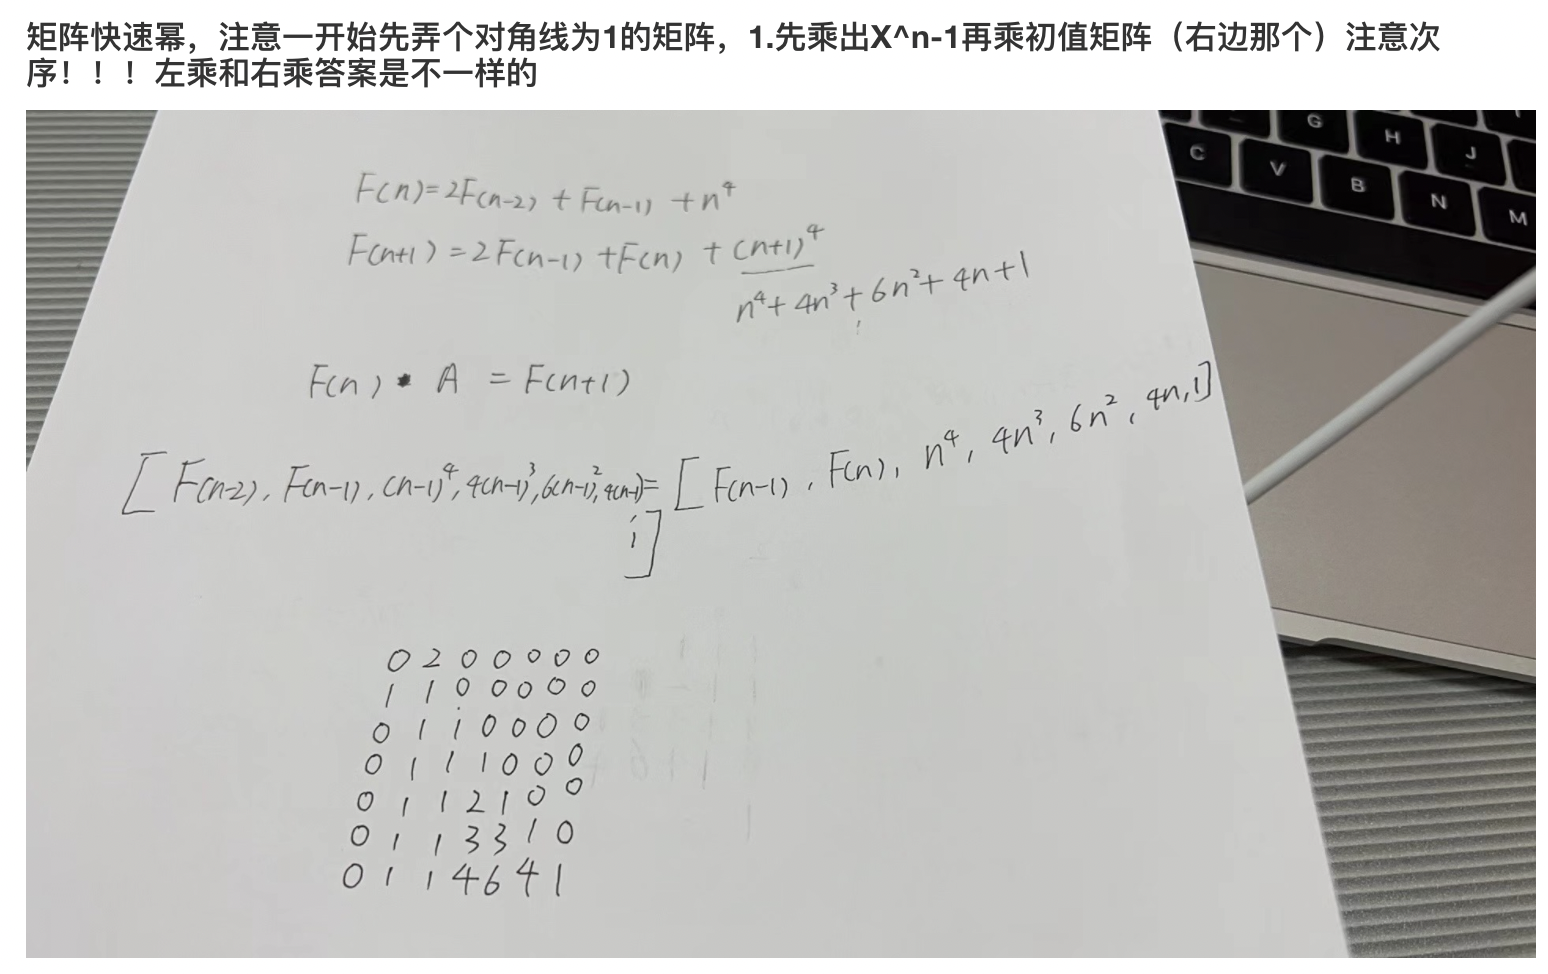
\includegraphics[scale=0.6]{数论/矩阵.png}
\inputminted[breaklines]{c++}{数论/矩阵快速幂.cpp}
\subsection{筛质数} % 二级标题
\subsubsection{线性筛(欧拉函数)} % 三级标题
\inputminted[breaklines]{c++}{数论/线性筛求欧拉函数.cpp}
\subsection{组合数} % 二级标题
\subsubsection{杨辉三角} % 三级标题
\inputminted[breaklines]{c++}{数论/杨辉三角.cpp}
\subsubsection{lucas定理($a,b\le10^{18}$)P是质数} % 三级标题
\inputminted[breaklines]{c++}{数论/lucas.cpp}
\subsubsection{扩展lucas($a,b\le10^{18}$)P不一定质数} % 三级标题
\inputminted[breaklines]{c++}{数论/扩展lucas.cpp}
\subsection{卡特兰数的应用}
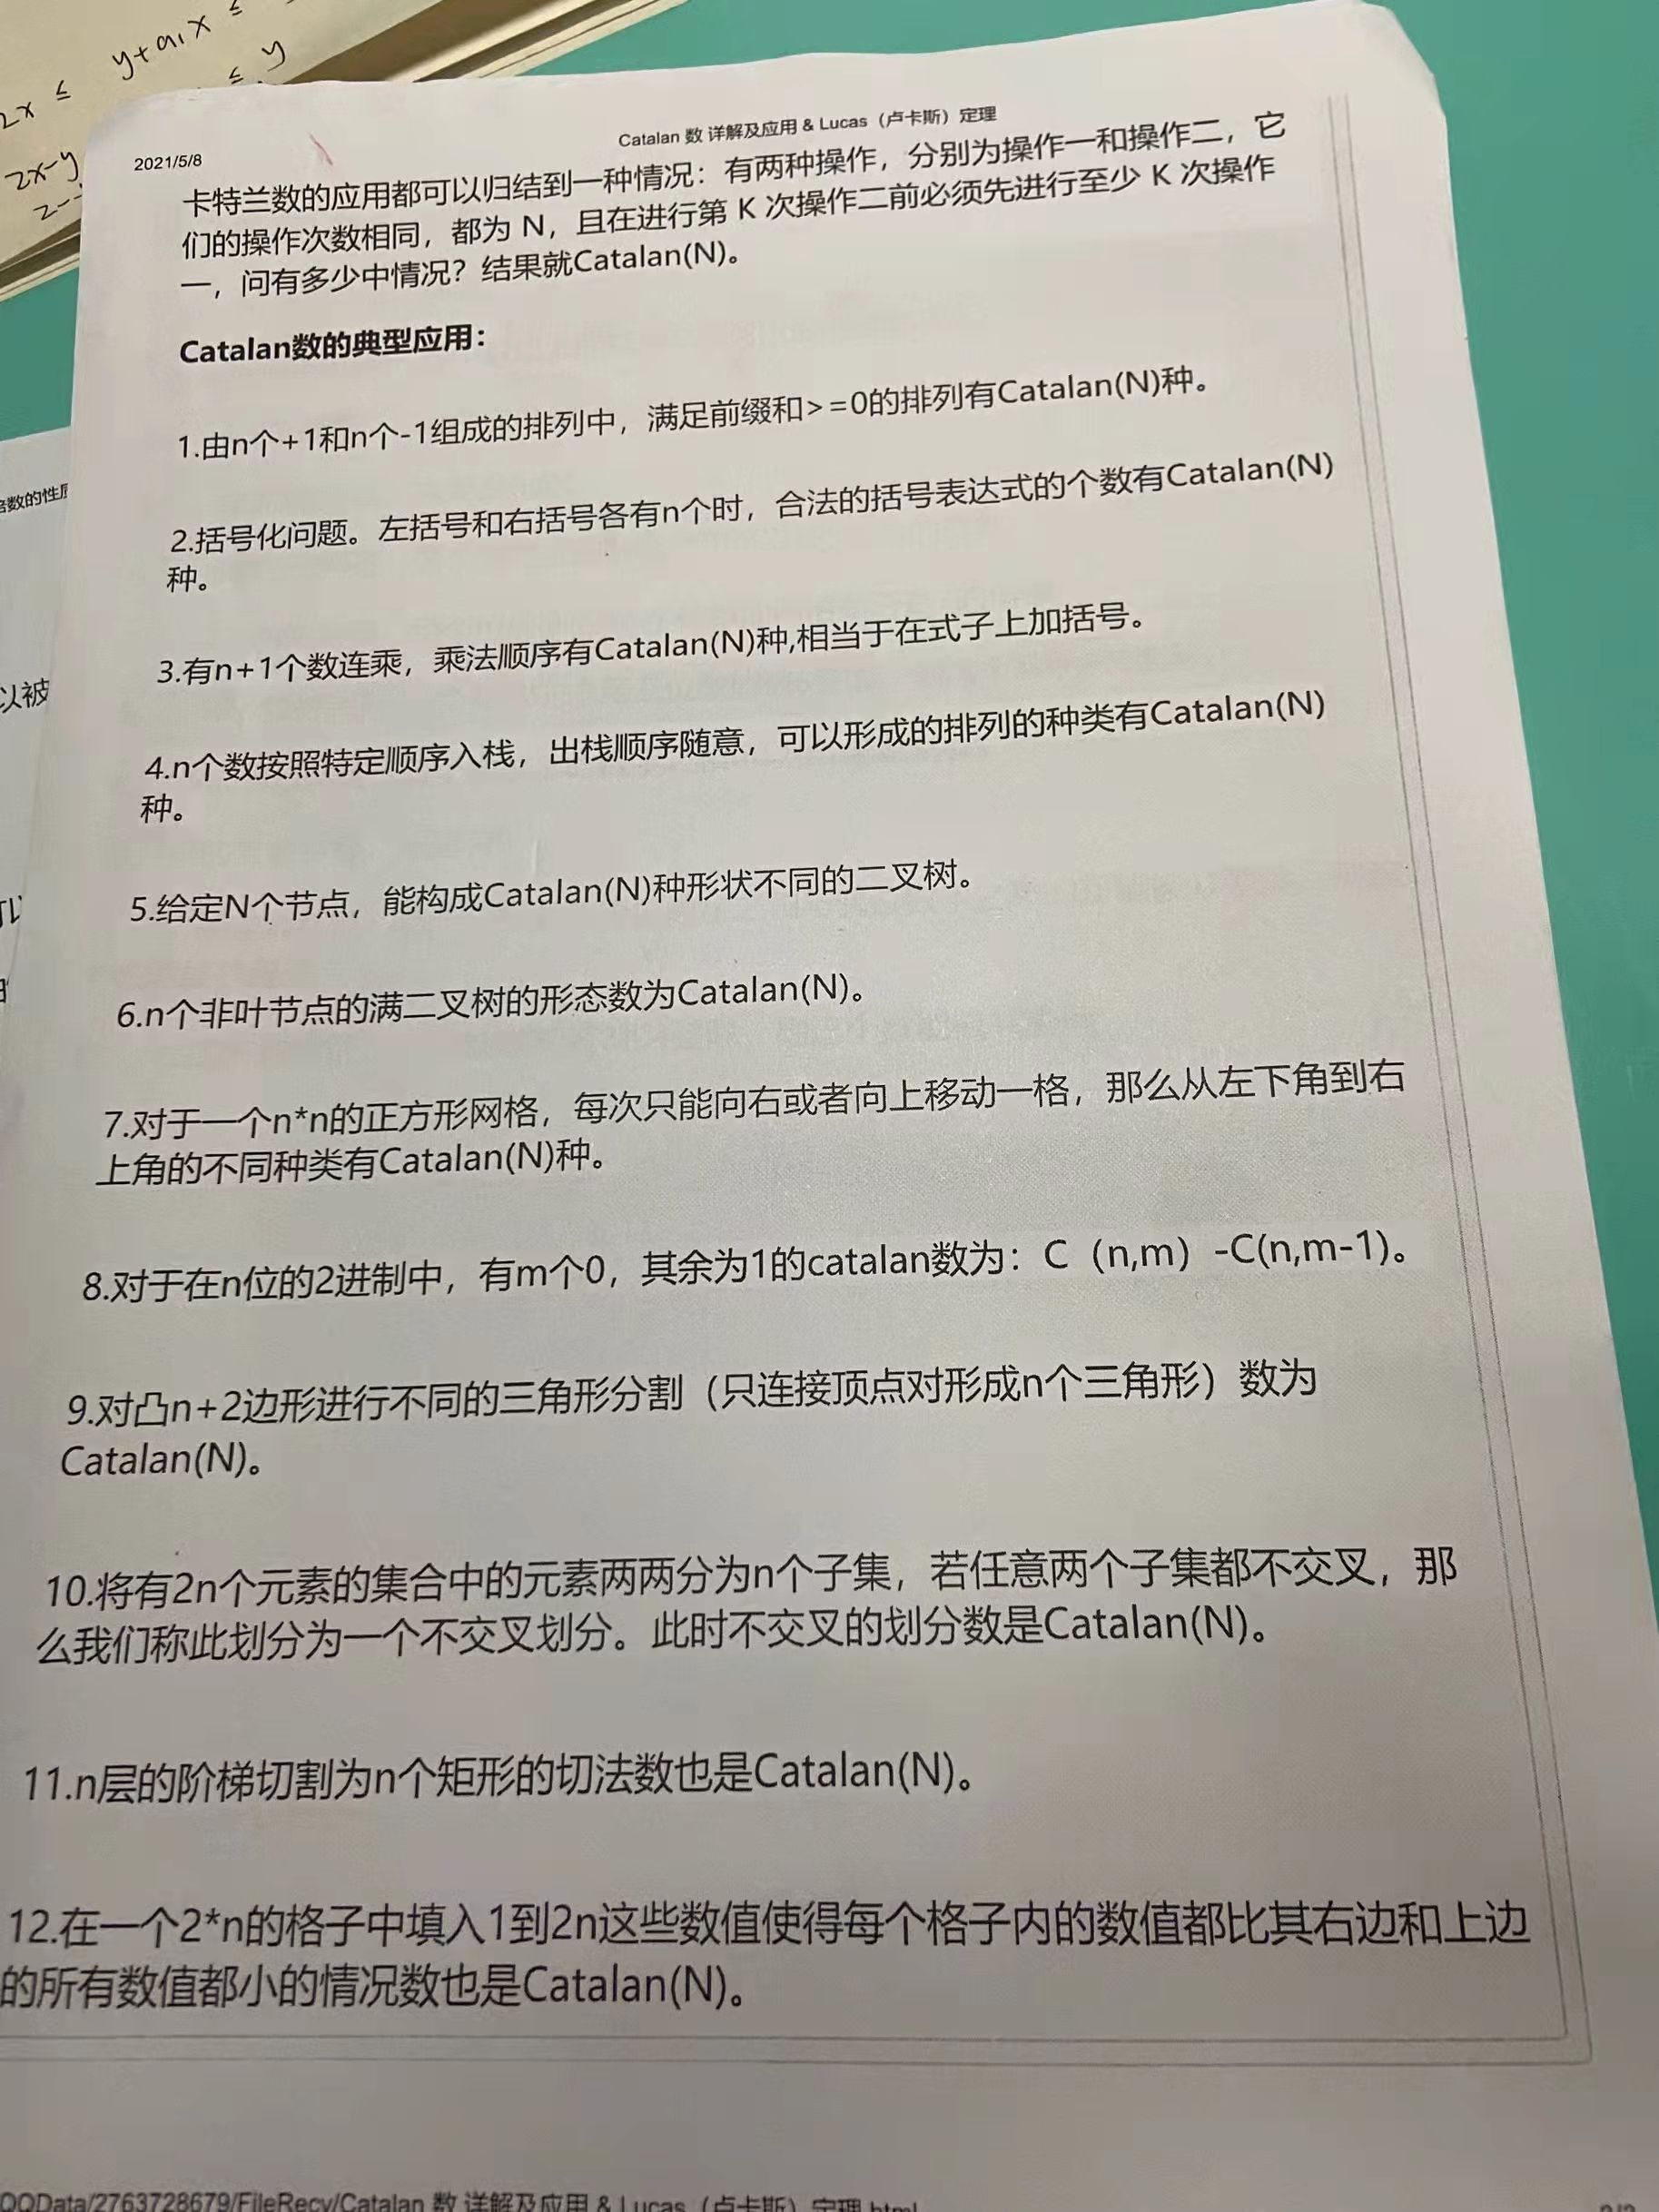
\includegraphics[scale=0.6]{数论/卡特兰数应用.png}
\subsubsection{卡特兰数(P可能是合数,阶乘分解法)} % 三级标题
\inputminted[breaklines]{c++}{数论/卡特兰数.cpp}
\subsection{约数} % 二级标题
\subsubsection{约数个数} % 三级标题
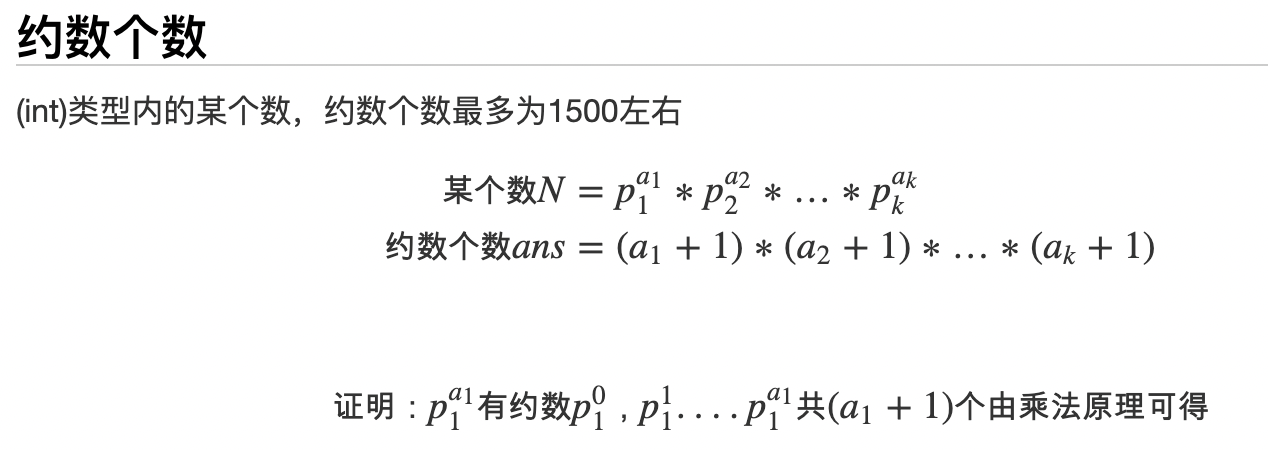
\includegraphics[scale=0.6]{数论/约数个数.png}
\inputminted[breaklines]{c++}{数论/约数个数.cpp}
\subsubsection{约数的和} % 三级标题
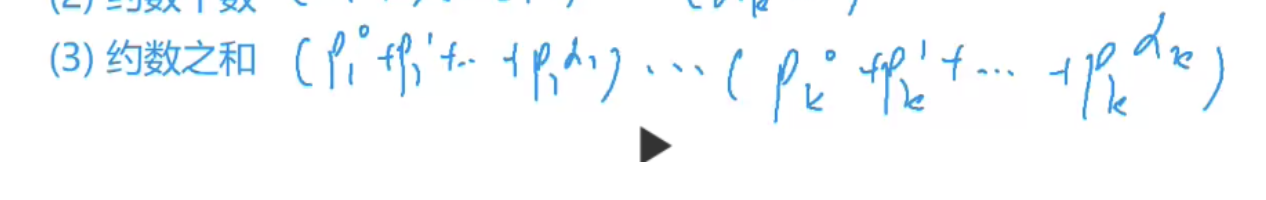
\includegraphics[scale=0.6]{数论/约数的和.png}
\inputminted[breaklines]{c++}{数论/约数的和.cpp}
\subsection{Exgcd及同余性质} % 二级标题
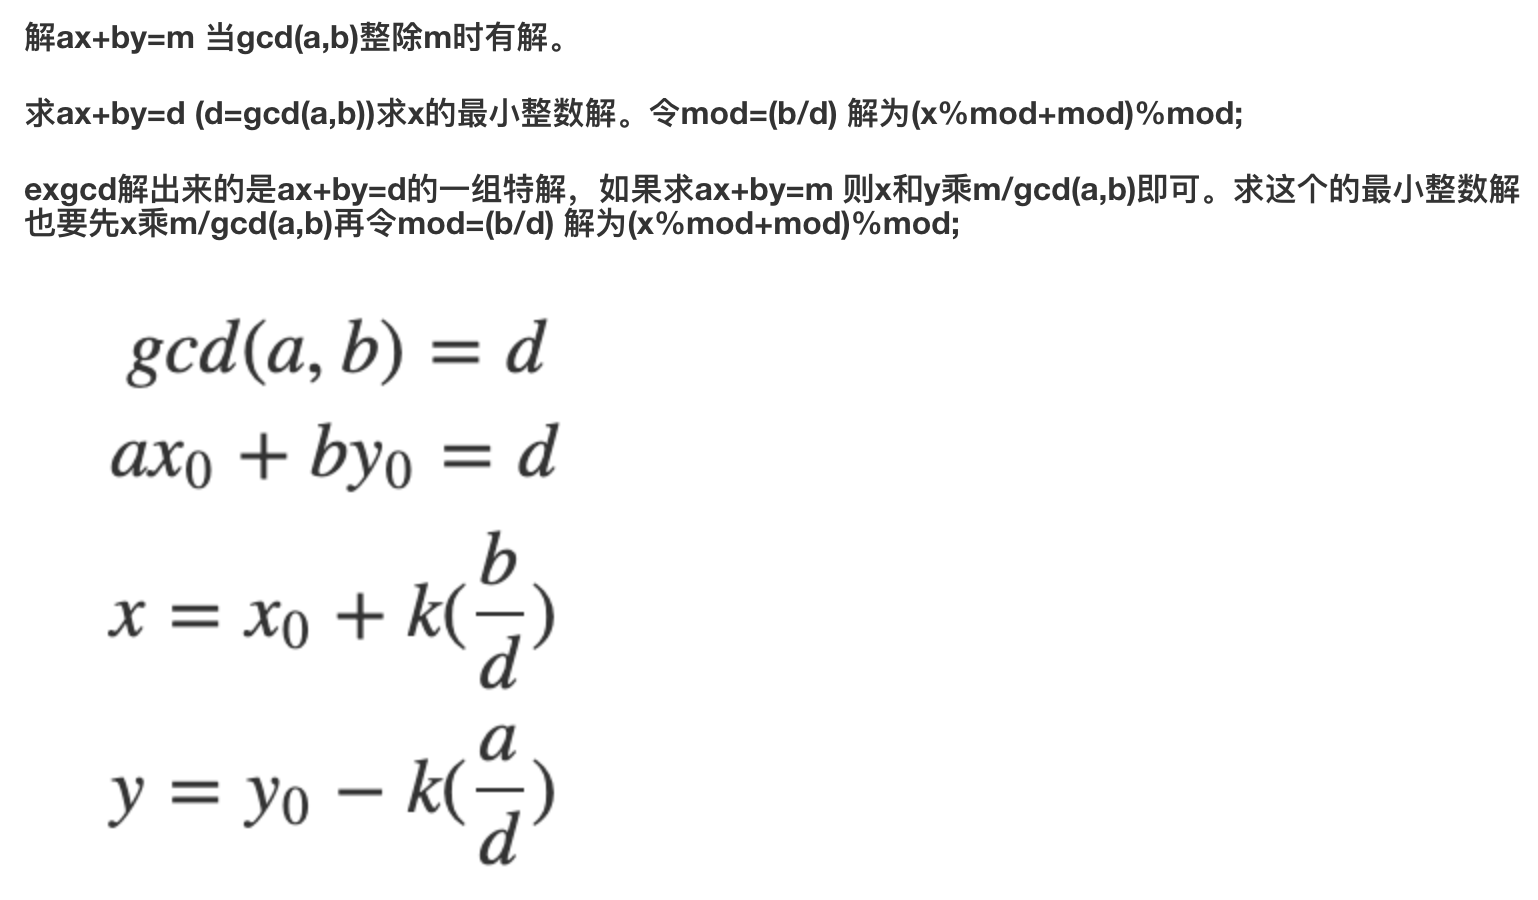
\includegraphics[scale=0.6]{数论/exgcd1.png}
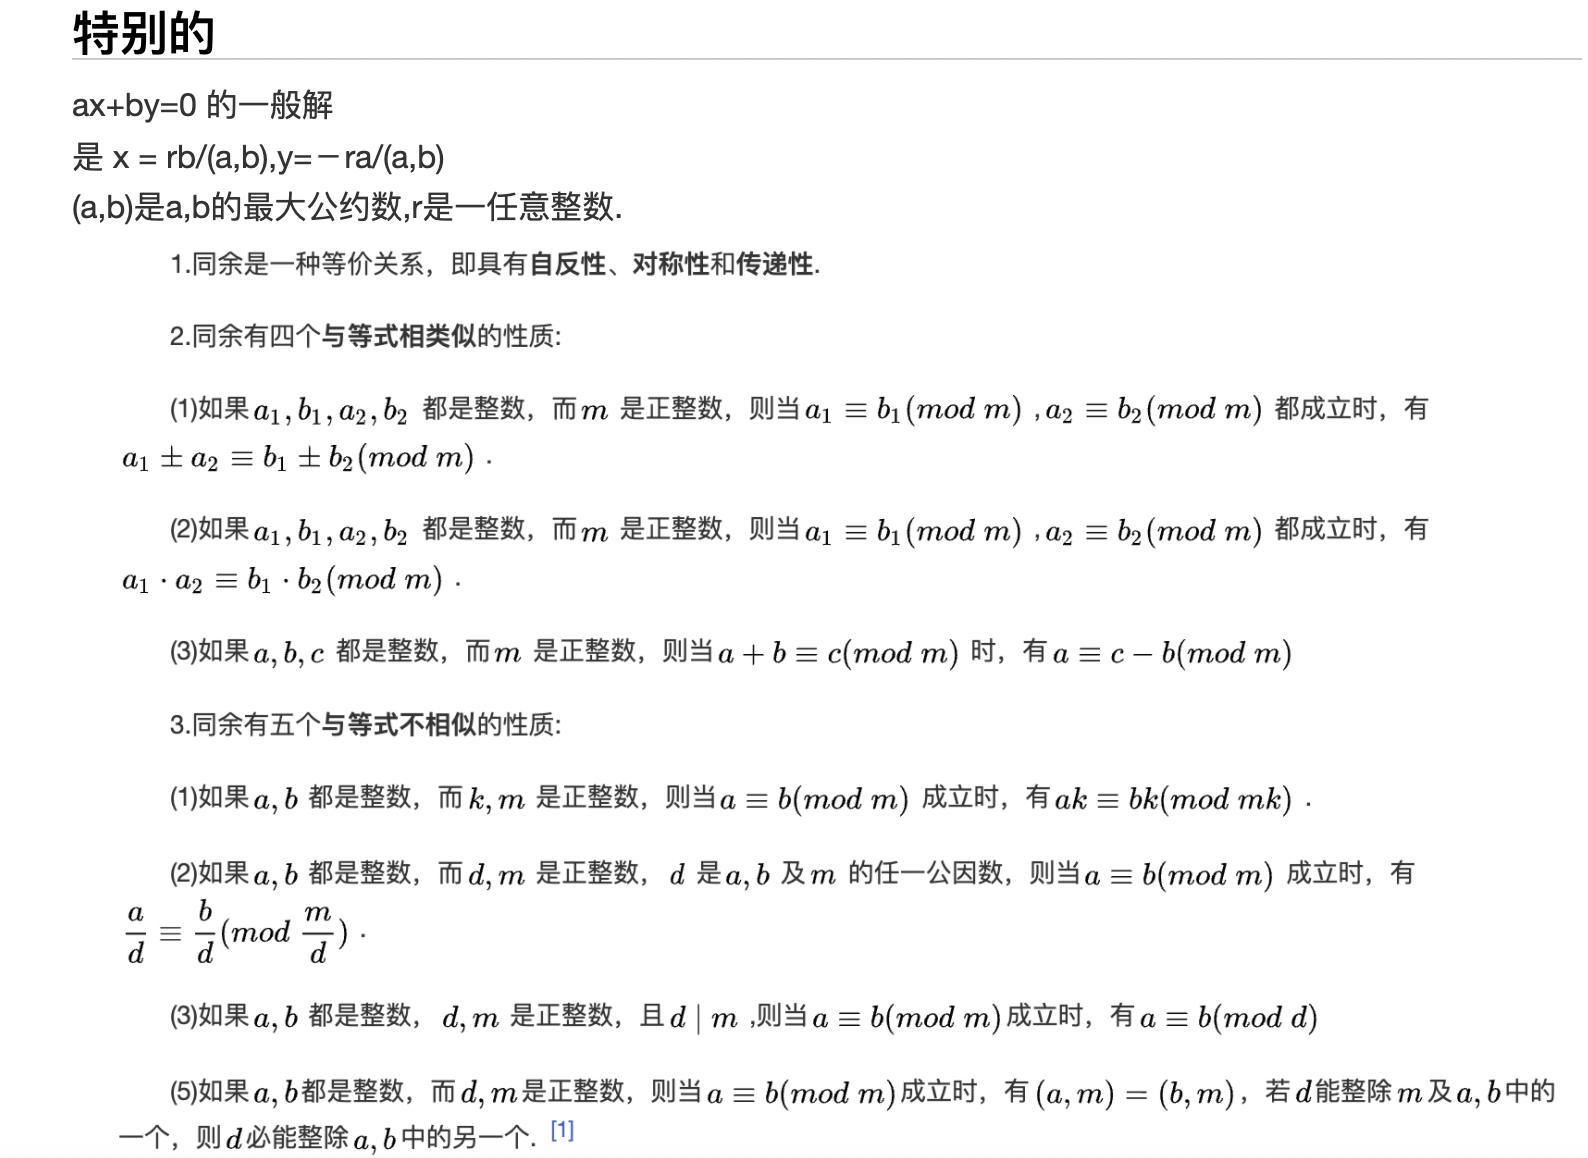
\includegraphics[scale=0.6]{数论/exgcd2.png}
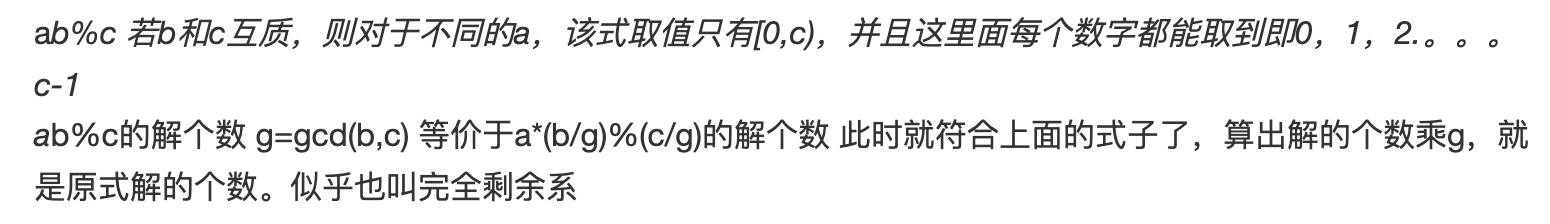
\includegraphics[scale=0.6]{数论/exgcd3.png}
\inputminted[breaklines]{c++}{数论/exgcd.cpp}
\subsection{高斯消元$n^3$} % 二级标题
\subsubsection{高斯消元解齐次线性方程组} % 三级标题
\inputminted[breaklines]{c++}{数论/高斯消元.cpp}
\subsubsection{高斯消元解异或线性方程组} % 三级标题
\inputminted[breaklines]{c++}{数论/高斯消元解异或线性方程组.cpp}
\subsubsection{高斯消元求行列式值(取模/double)} % 三级标题
\inputminted[breaklines]{c++}{数论/高斯消元求行列式值.cpp}
\subsection{容斥原理} % 二级标题
\inputminted[breaklines]{c++}{数论/容斥原理.cpp}
\subsection{FFT与NTT} % 二级标题
\inputminted[breaklines]{c++}{数论/FFT.cpp}
\subsection{BSGS(普通和扩展)} % 二级标题
\inputminted[breaklines]{c++}{数论/BSGS.cpp}
\subsection{生成函数} % 二级标题
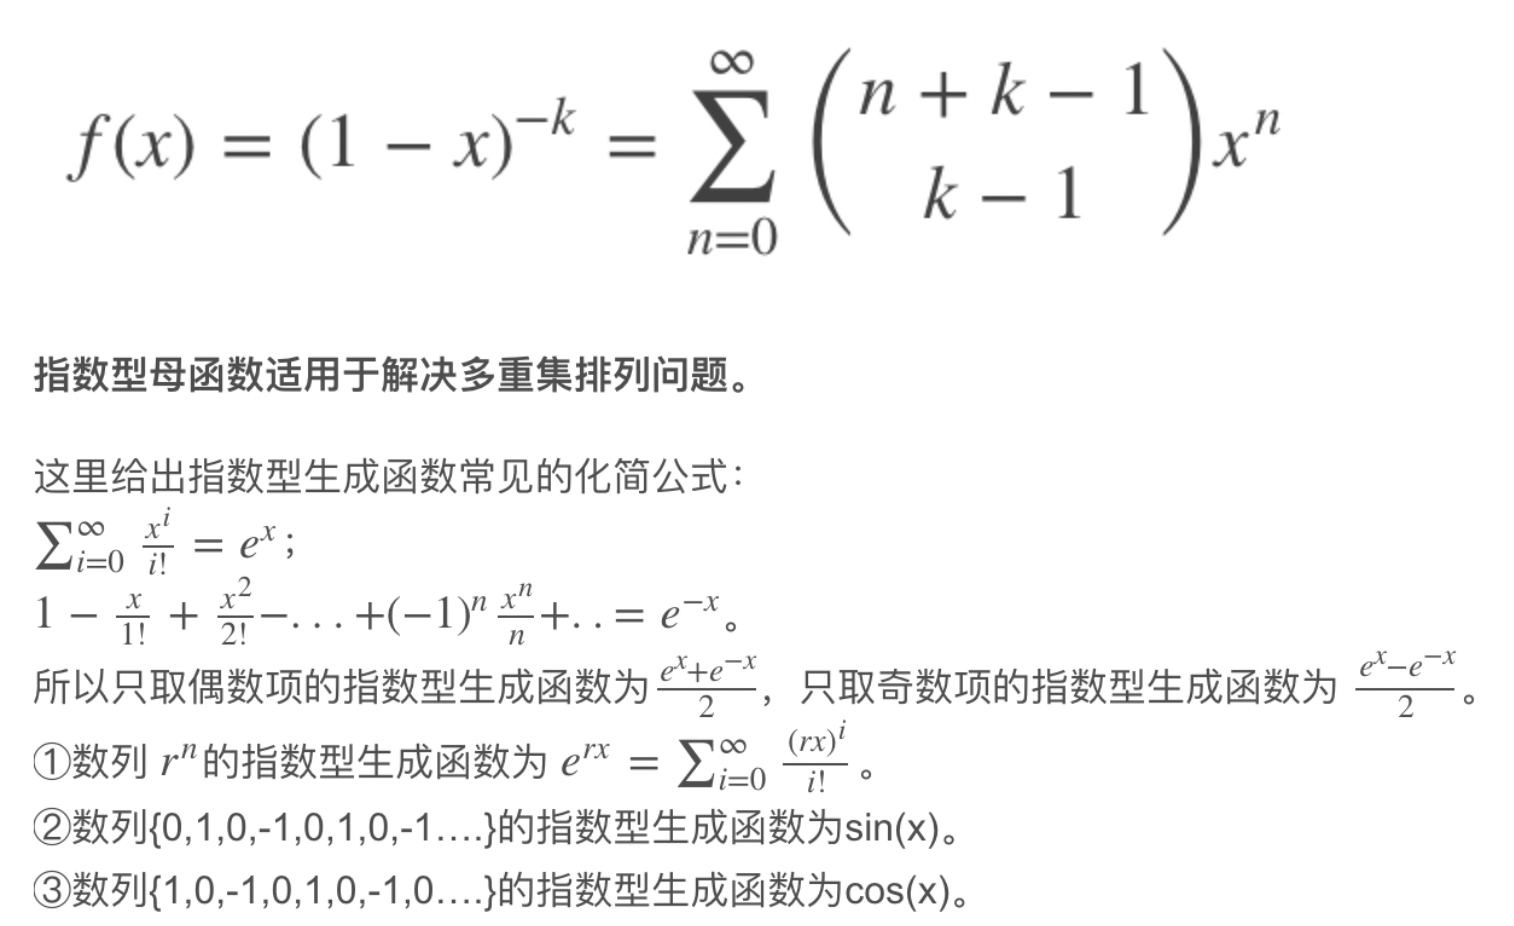
\includegraphics[scale=0.6]{数论/生成函数1.png}
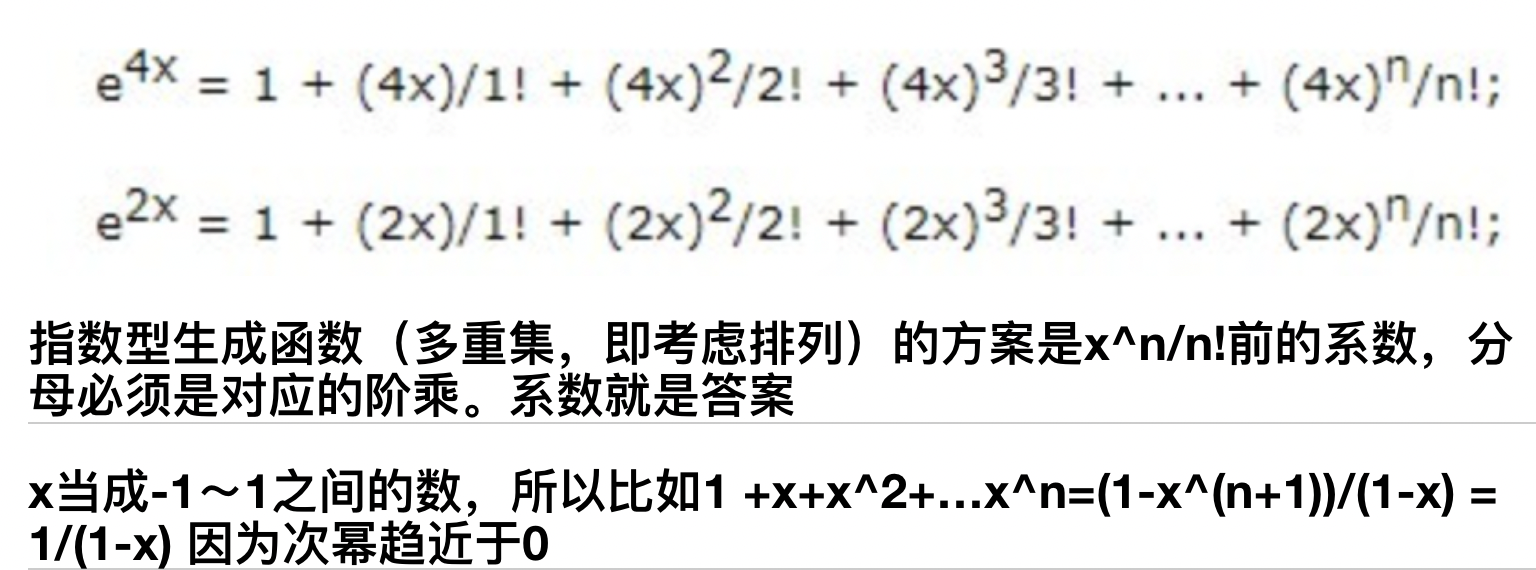
\includegraphics[scale=0.6]{数论/生成函数2.png}
\subsection{线性基} % 二级标题
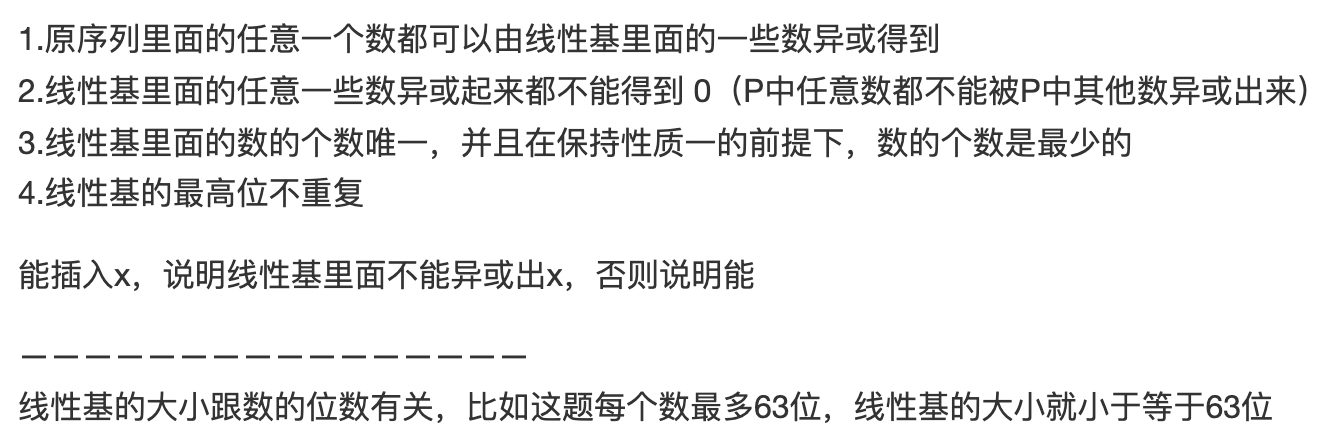
\includegraphics[scale=0.6]{数论/线性基.png}
\inputminted[breaklines]{c++}{数论/线性基.cpp}
\subsection{欧拉降幂} % 二级标题
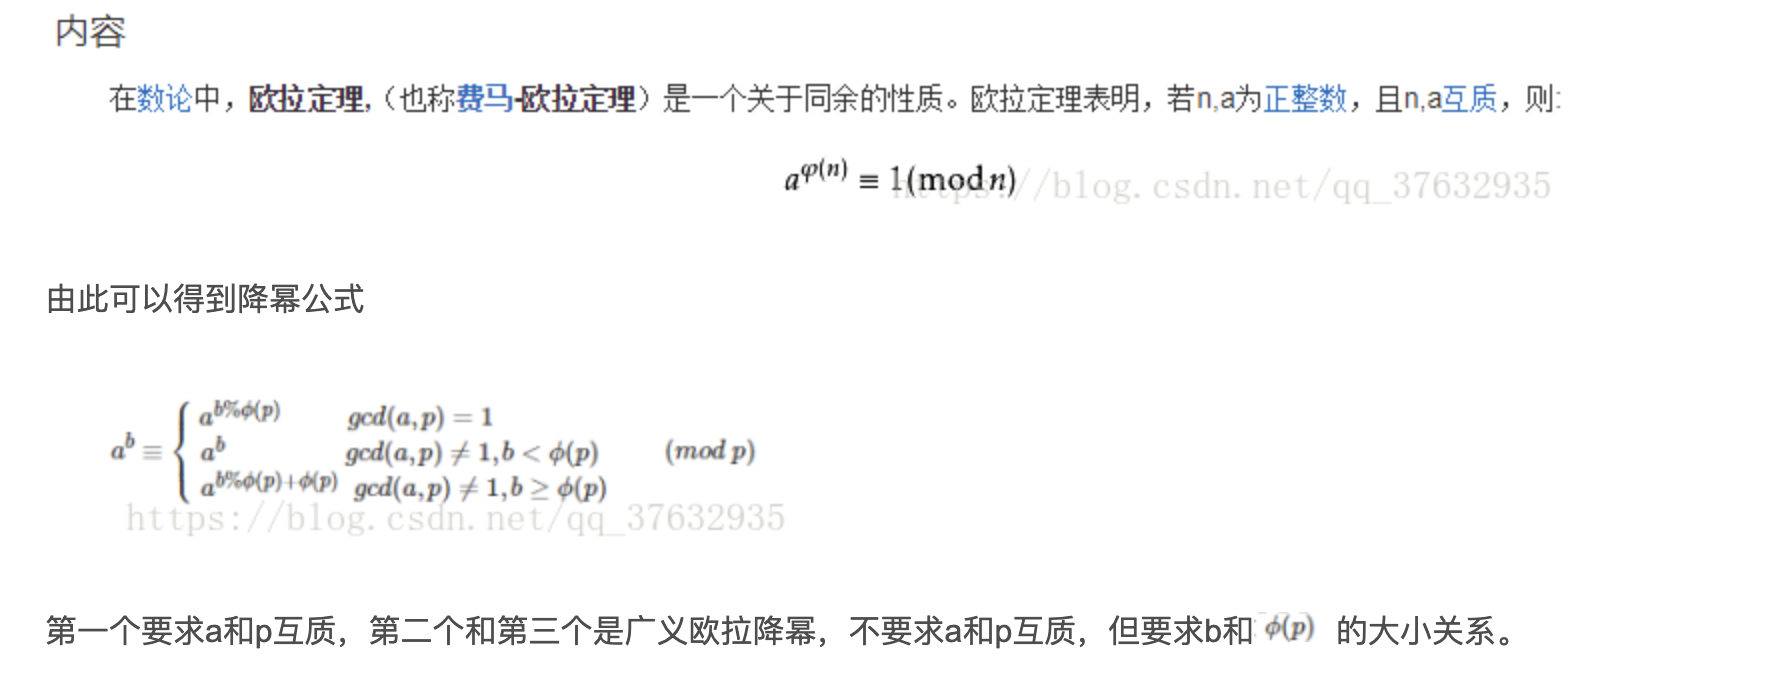
\includegraphics[scale=0.6]{数论/欧拉降幂.png}
\inputminted[breaklines]{c++}{数论/欧拉降幂.cpp}
\subsection{康托展开求排列的字典序排名}
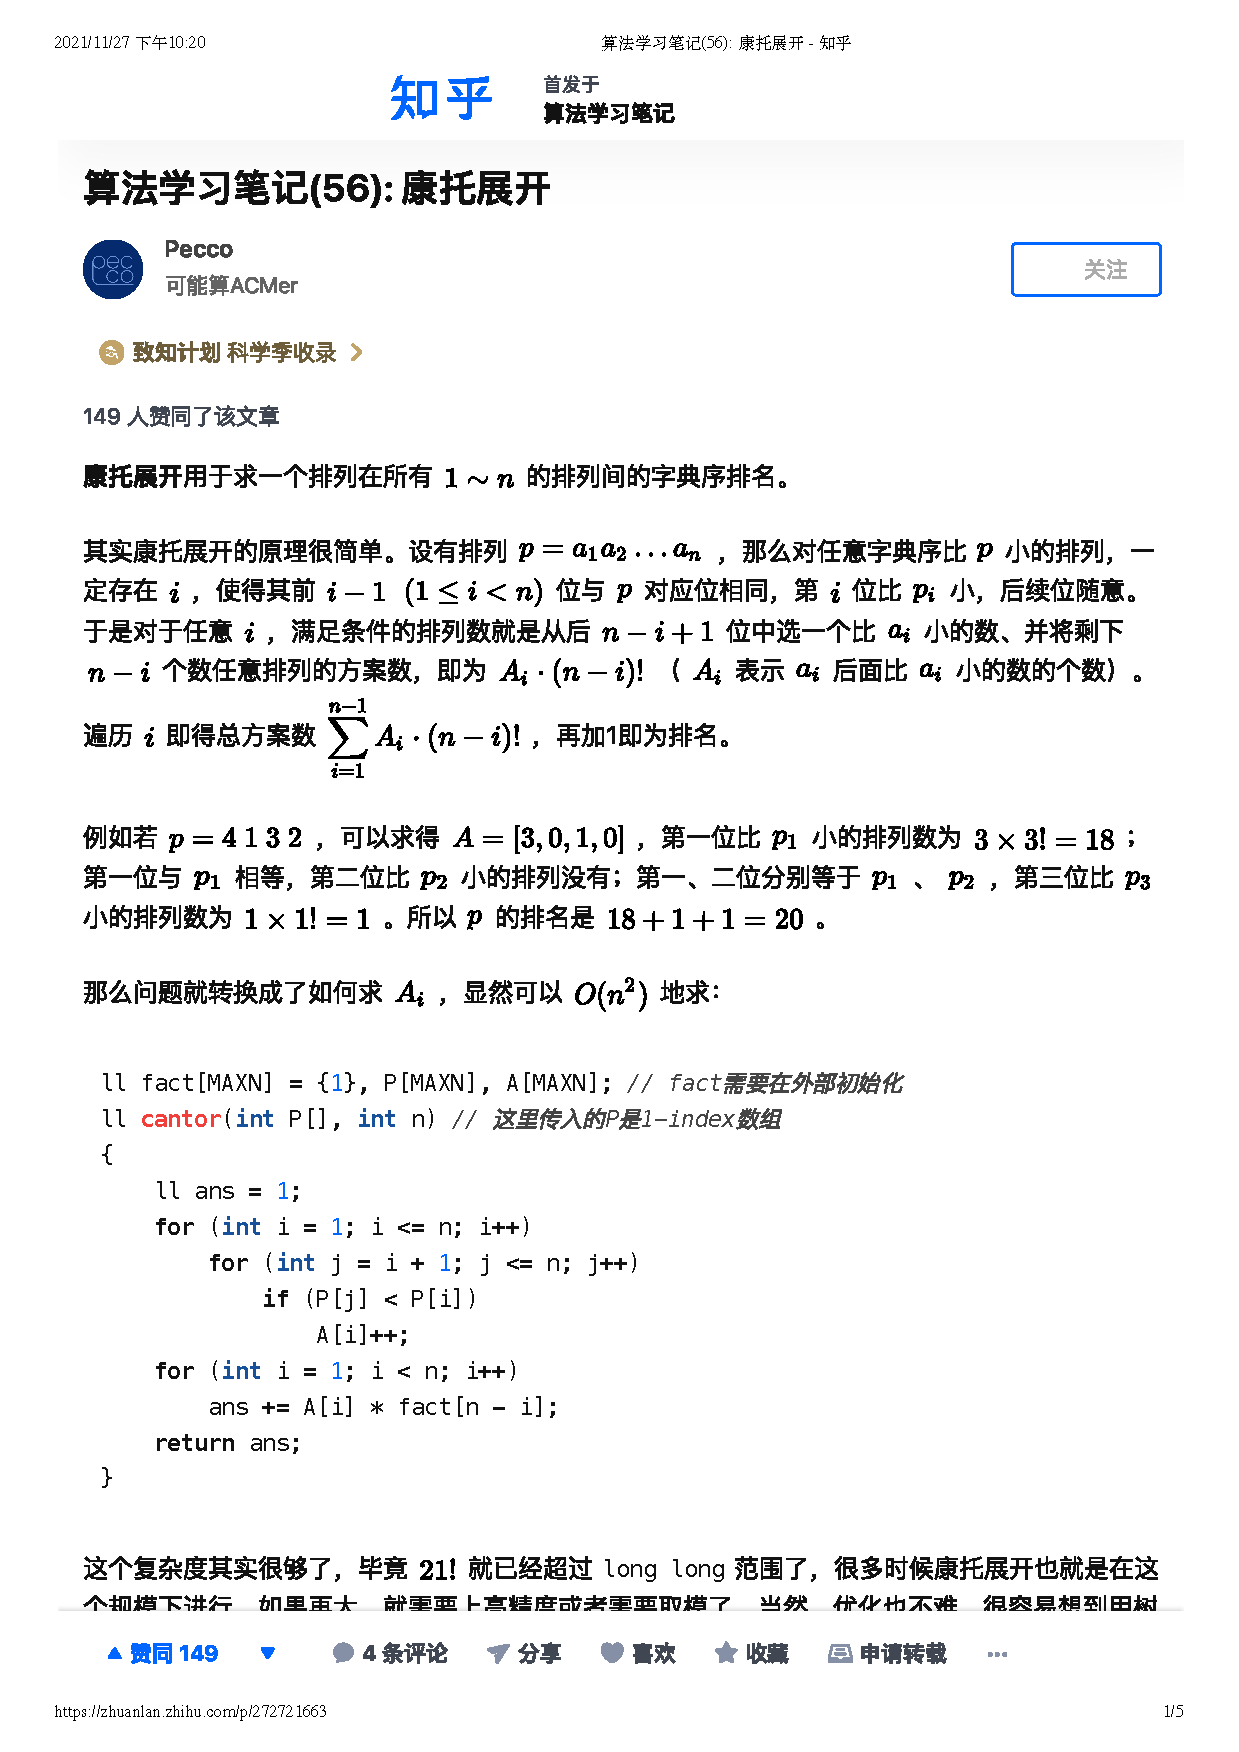
\includepdf[pages={1,2,3}]{数论/康托展开.pdf}

\newpage
\section{计算几何} % 一级标题
\subsection{凸包} % 二级标题
\inputminted[breaklines]{c++}{计算几何/凸包.cpp}
\subsection{半平面交} % 二级标题
\inputminted[breaklines]{c++}{计算几何/半平面交.cpp}
\subsection{最小圆覆盖} % 二级标题
\inputminted[breaklines]{c++}{计算几何/最小圆覆盖.cpp}
\subsection{三维凸包} % 二级标题
\inputminted[breaklines]{c++}{计算几何/三维凸包.cpp}
\subsection{旋转卡壳} % 二级标题
\subsubsection{平面最远点对} % 三级标题
\inputminted[breaklines]{c++}{计算几何/旋转卡壳.cpp}
\subsubsection{最小矩形覆盖} % 三级标题
\inputminted[breaklines]{c++}{计算几何/最小矩形覆盖.cpp}
\subsection{三角剖分(圆和多边形面积交)} % 二级标题
\inputminted[breaklines]{c++}{计算几何/三角剖分.cpp}
\subsection{扫描线} % 二级标题
\subsubsection{三角形面积并} % 三级标题
\inputminted[breaklines]{c++}{计算几何/三角形面积并.cpp}
\subsubsection{矩形面积并} % 三级标题
\inputminted[breaklines]{c++}{计算几何/矩形面积并.cpp}
\subsection{自适应辛普森积分} % 二级标题
\inputminted[breaklines]{c++}{计算几何/自适应辛普森积分.cpp}

%\twocolumn  % 分页显示
\newpage
\section{字符串}
\subsection{字符串哈希}
\inputminted[breaklines]{c++}{字符串/字符串哈希.cpp}
\subsection{KMP}
\inputminted[breaklines]{c++}{字符串/kmp.cpp}
\subsection{EXKMP}
\inputminted[breaklines]{c++}{字符串/exkmp.cpp}
\subsection{manacher}
\inputminted[breaklines]{c++}{字符串/manacher.cpp}
\subsection{AC自动机}
\inputminted[breaklines]{c++}{字符串/ac自动机.cpp}
\subsection{后缀自动机}
\inputminted[breaklines]{c++}{字符串/后缀自动机.cpp}
\subsection{后缀数组}
\inputminted[breaklines]{c++}{字符串/后缀数组.cpp}

\newpage
\section{博弈论} % 一级标题
\subsection{SG函数} % 二级标题
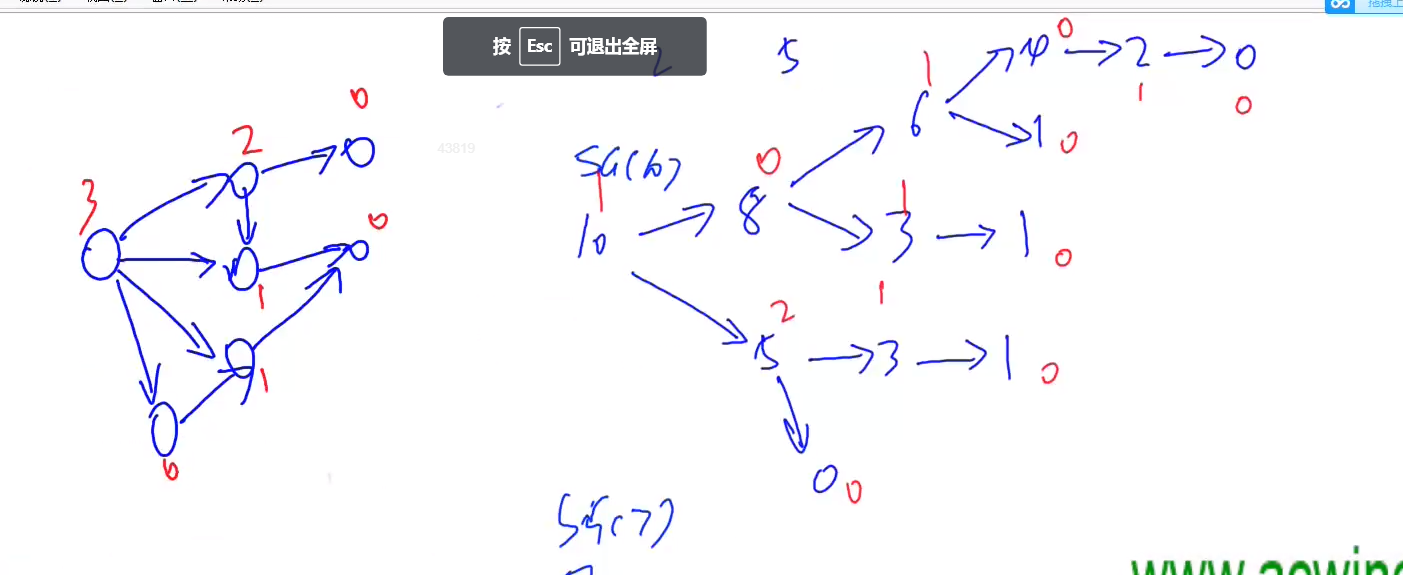
\includegraphics[scale=0.3]{博弈论/sg.png}
\inputminted[breaklines]{c++}{博弈论/sg函数.cpp}

\newpage
\section{混合板子}
\subsection{杜教BM(求线性递推)}
\inputminted[breaklines]{c++}{混合板子/杜教BM.cpp}
\subsection{complex复数板子}
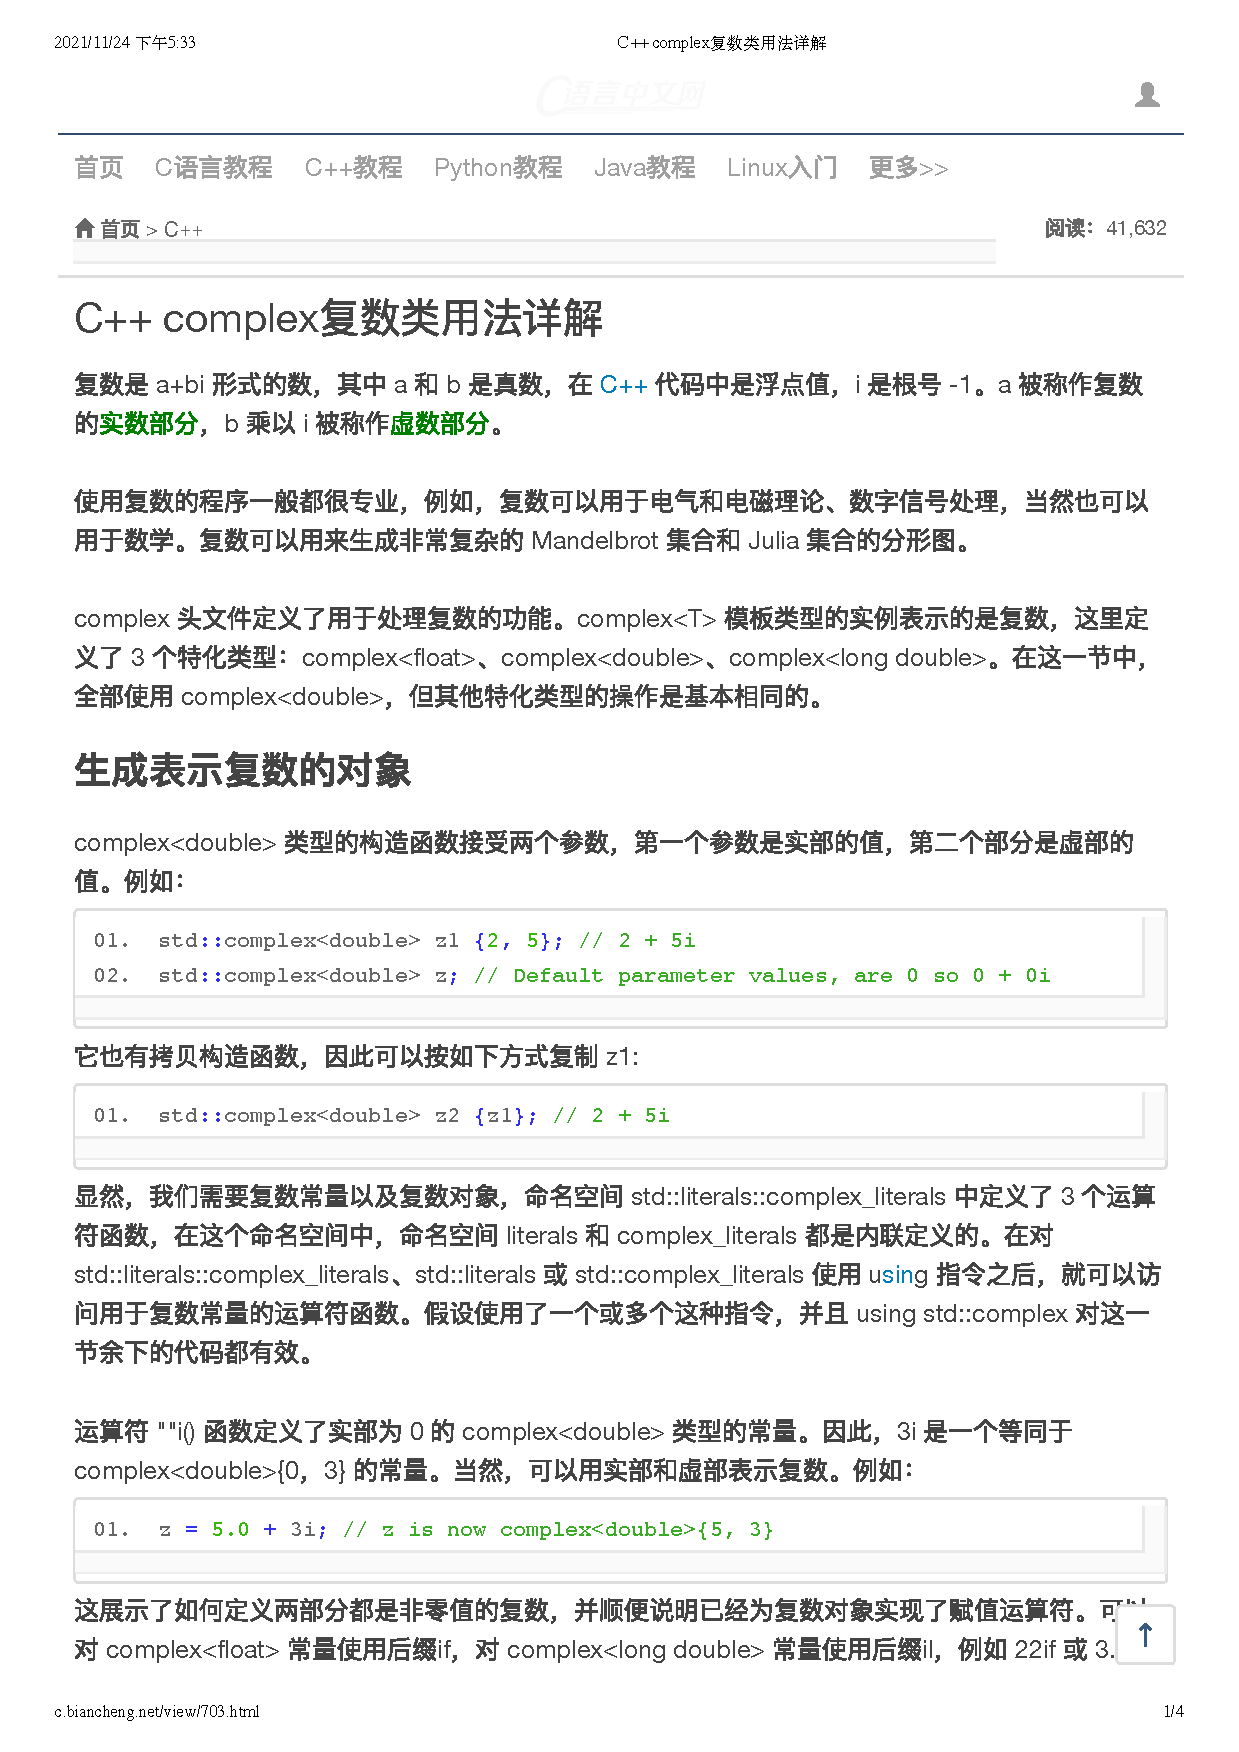
\includepdf[pages={1,2,3}]{混合板子/complex.pdf}
\subsection{快读}
\inputminted[breaklines]{c++}{混合板子/快读.cpp}
\subsection{随机与cin解绑}
\inputminted[breaklines]{c++}{混合板子/随机与解绑.cpp}
%\newpage
%\section{Others}

\end{document}
